\chapter{Pruebas de escala}

% **************************** Define Graphics Path **************************
\graphicspath{{Chapter4/Figs/}}

Con el entorno de simulación construido, el siguiente objetivo es realizar pruebas de escala sobre la arquitectura. Se realizan dos tipos de pruebas de escala: (a) verificar cómo funciona la arquitectura para topologias de escala, (b) realizar estudios de escala sobre la cantidad de servicios que soporta. En este capítulo se explicará el propósito de cada prueba, las condiciones bajo las cuales se ejecuta cada una de ellas (topologias, tipos de tráfico, etc) y por último, los resultados que arrojan. Las pruebas fueron realizadas en el servidor del Instituto de Computación, con una máquina virtual Lubuntu 14.04 sobre KVM, con 32GB de RAM y un procesador AMD Opteron 23xx.

\section{Topologias de escala}
Como se explica en el capítulo 1, la arquitectura RAUFlow ha sido probada (hasta antes de realizar este trabajo) con una topología de 4 nodos, debido a las limitaciones del prototipo físico. Por lo tanto, el objetivo de estas pruebas es utilizar el entorno virtual para aplicar topologias de diferentes tamaños y características a la arquitectura y estudiar el proceso de creación de las redes privadas virtuales en cada realidad.

Es importante tener en cuenta que realizar esta serie de pruebas es posible gracias al proceso de verificación funcional explicado en la sección 3.5. En ella se explica la detección y corrección de algunos problemas de escalabilidad tanto del entorno virtual como de la arquitectura RAUFlow misma. Por lo tanto, estas pruebas se pueden considerar como una continuación del estudio de escalabilidad presentado en dicha sección.

\subsection{Descripción del escenario}

Las topologias utilizadas se listan a continuación:
\begin{itemize}
	\item \textbf{Básica}: 4 nodos en topología de full mesh. Es la utilizada en el prototipo físico. Figura \ref{fig:basic_topology}.
	\item \textbf{Chica}: topología arbitraria de 11 nodos (fuente: Topology Zoo). Figura \ref{fig:small_topology}.
	\item \textbf{Mediana}: topología arbitraria de 45 nodos (fuente: Topology Zoo). Figura \ref{fig:medium_topology}.
	\item \textbf{Grande}: topología de tipo arborescente compuesta por 105 nodos. Figura \ref{fig:large_topology}
\end{itemize}

Todas las topologias tienen las siguientes características:
\begin{itemize}
	\item Tienen un conjunto de RAUSwitch, conectados de acuerdo a lo que dicte la topología.
	\item Existen dos subredes cliente, implementadas por un QuaggaRouter y un RAUHost cada una (recordar las clases del entorno virtual). El RAUHost representa la computadora que utiliza el usuario final para conectarse a la red, y QuaggaRouter representa el router legacy que conecta la subred del usuario a la red SDN. Los RAUHost serán los remitentes y destinatarios del tráfico que pasará por la red. Esos datos se generarán con el comando \textit{ping} y la herramienta \textit{iperf}. Estas dos subredes tendrán una ubicación variable en cada topología, ya que se probará con distintos caminos entre ellas. Por esta razón, se omiten en las imágenes de las topologias.
	\item El controlador se conecta con un switch virtual genérico (implementado por la clase Switch de Mininet, en el modo \textit{standalone}), el cual se conecta con los RAUSwitch. Esta será la red de gestión. Por simplicidad, dicha red se omite en las imágenes.
\end{itemize}

\begin{figure}[H]
	\caption{Topología de prueba básica}
	\includegraphics[scale=0.6]{basic_topology}
	\centering
	\label{fig:basic_topology}
\end{figure}

\begin{figure}[H]
	\caption{Topología de prueba chica}
	\includegraphics[scale=0.4]{small_topology}
	\centering
	\label{fig:small_topology}
\end{figure}

\begin{figure}[H]
	\caption{Topología de prueba mediana}
	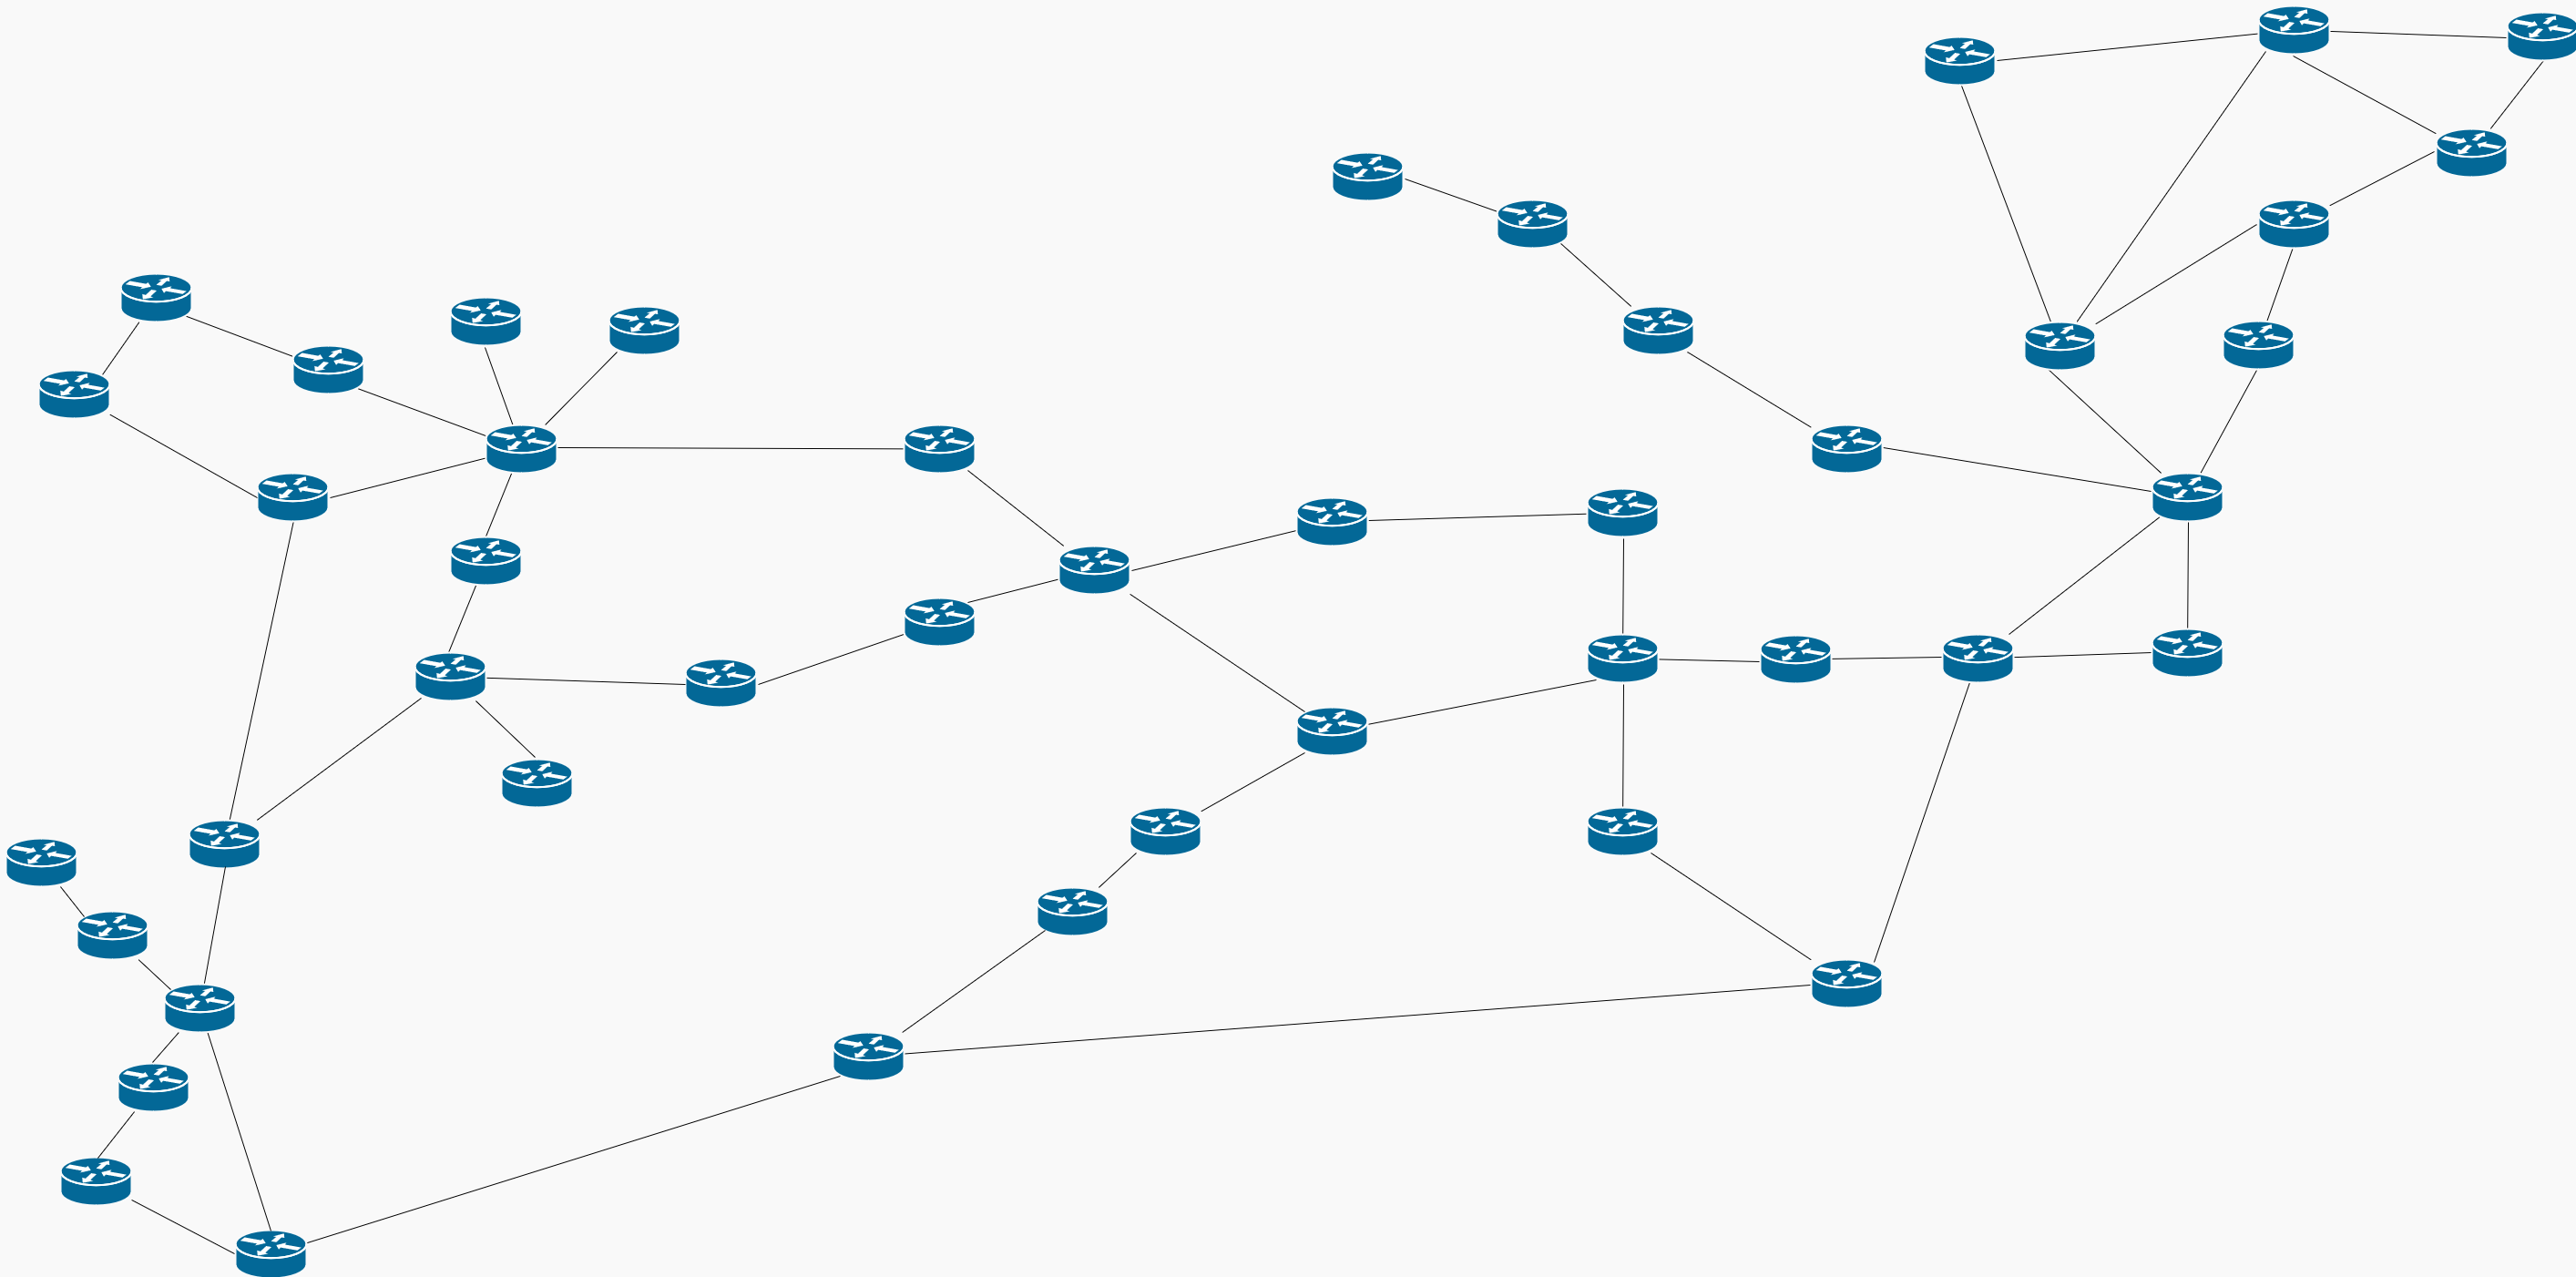
\includegraphics[width=\textwidth,height=\textheight,keepaspectratio]{medium_topology}
	\centering
	\label{fig:medium_topology}
\end{figure}

\begin{figure}[H]
	\caption{Topología de prueba grande}
	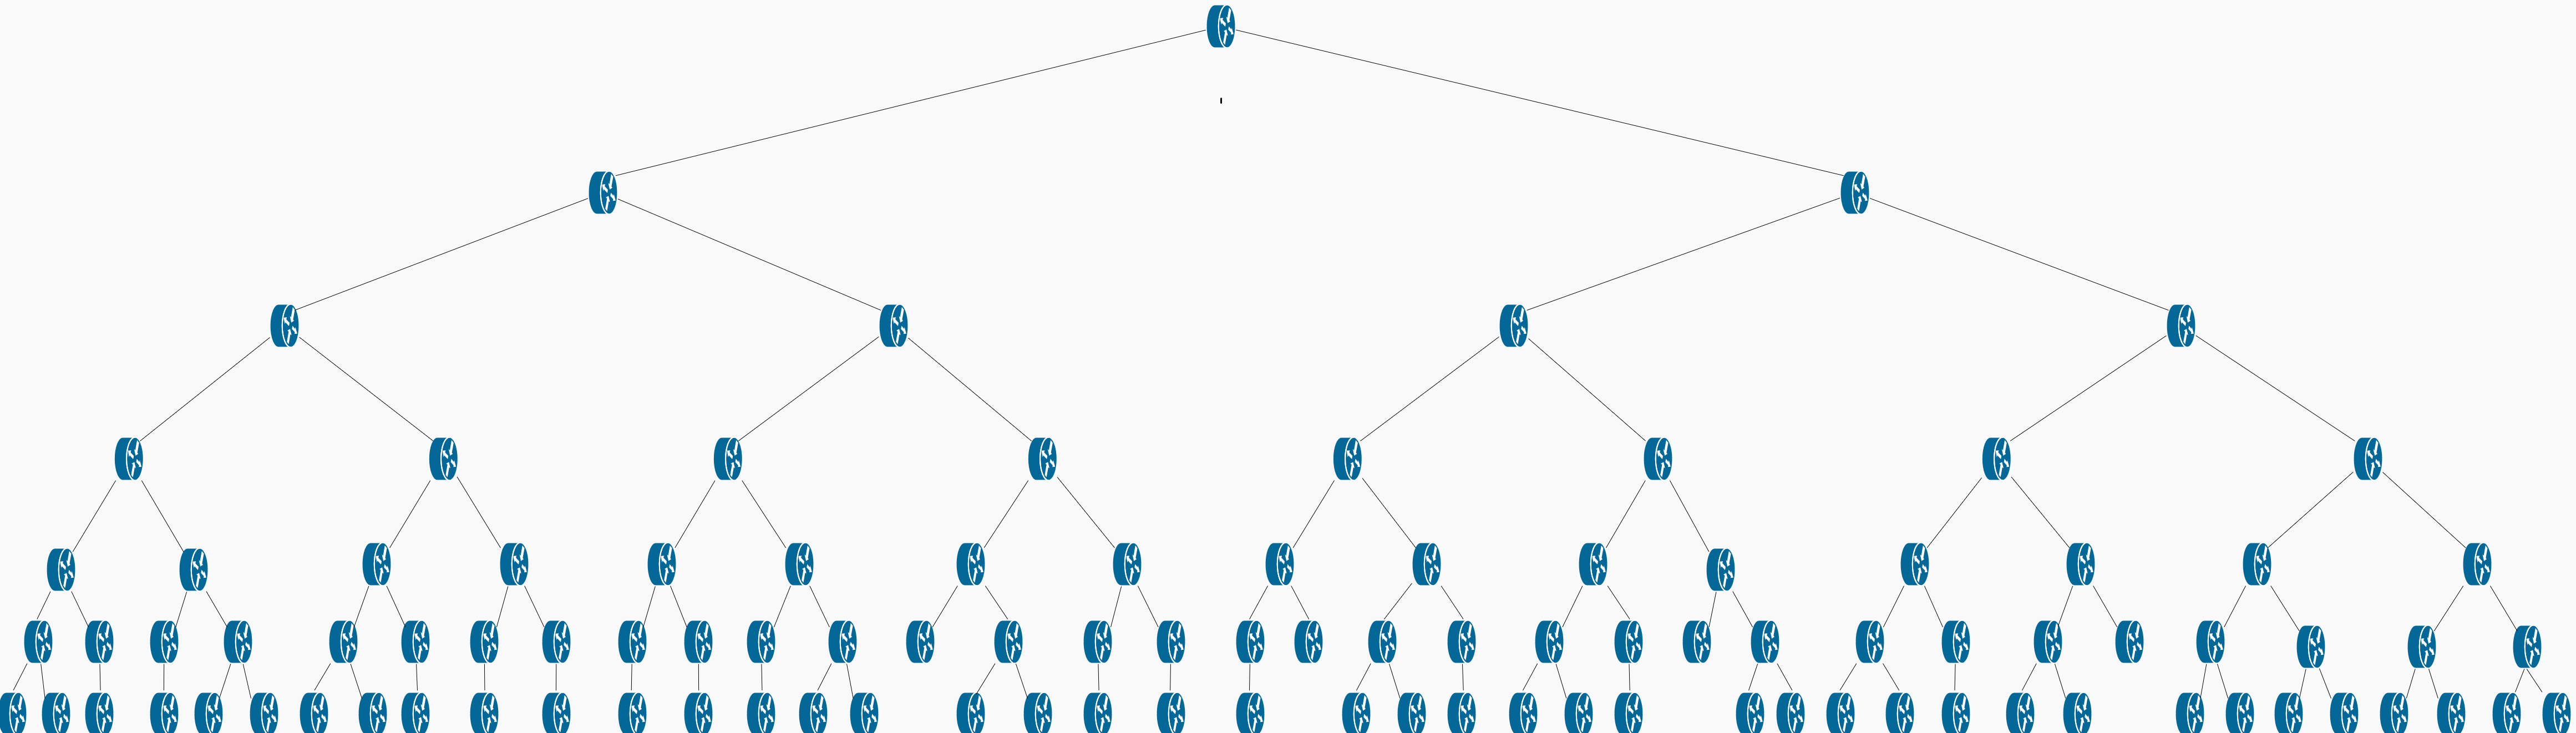
\includegraphics[width=\textwidth,height=\textheight,keepaspectratio]{large_topology}
	\centering
	\label{fig:large_topology}
\end{figure}

El objetivo es estudiar como impacta el tamaño de la topología y el largo del camino en el tiempo que demora la arquitectura en establecer una VPN entre dos subredes cliente. Se espera que ese tiempo sea influenciado en gran medida por dos factores: el tiempo que demora el controlador en calcular el camino óptimo y el tiempo que demora en configurar los flujos en cada nodo del camino. Dado que los servicios se crean enviando pedidos HTTP POST al controlador (y se deben enviar dos por cada VPN, uno de ida y uno de vuelta), el tiempo de creación de los mismos se medirá como el tiempo que demore el controlador en devolver las respuestas HTTP indicando que fueron creados con éxito (esta información está disponible en los logs). Para lograr resultados representativos y reducir el margen de error, en lugar de crear una VPN y medir su tiempo solamente, se realizan cuatro ejecuciones y se calculan las métricas estadísticas relevantes. Para agilizar la ejecución de esta prueba se utiliza un script en Python que manda los pedidos HTTP POST al controlador para crear las VPN, y de este modo no hay necesidad de hacerlo manualmente a través de la interfaz web.

\subsection{Resultados y observaciones}

\newcolumntype{?}{!{\vrule width 3pt}}
\newcolumntype{M}[1]{>{\centering\arraybackslash}m{#1}}
\begin{table}
	\caption{Tiempo que demora el controlador en dar de alta VPNs. El tiempo se mide en ms. Los valores de color marrón  corresponden a la VPN de capa 2, y los azules a la de capa 3.}
	\centering
	\scriptsize
	\bgroup
	\setlength{\tabcolsep}{.17em}
	\begin{tabular}{M{1.1cm}? M{0.8cm} | M{1.7cm} | M{1.7cm} | M{1.7cm} | M{1.7cm} | M{1.5cm} | M{1.4cm} | M{1.3cm} | M{1.3cm} |@{}m{0pt}@{}}
		\Xhline{5\arrayrulewidth}
		Topología & Largo del camino & Ejecución 1 (ms) & Ejecución 2 (ms) & Ejecución 3 (ms) & Ejecución 4 (ms) & Media (ms) & Mediana (ms) & Desv. Estándar (ms) & CV & \\
		\hline
		Básica & 1 & \textcolor{brown}{188} / \textcolor{blue}{14} & \textcolor{brown}{188} / \textcolor{blue}{23} & \textcolor{brown}{199} / \textcolor{blue}{15} & \textcolor{brown}{188} / \textcolor{blue}{15} & \textcolor{brown}{191} / \textcolor{blue}{17} & \textcolor{brown}{188} / \textcolor{blue}{15} & \textcolor{brown}{6} / \textcolor{blue}{4} & \textcolor{brown}{0.03} / \textcolor{blue}{0.24} & \\[3ex]
		\Xhline{5\arrayrulewidth}
		& 1 & \textcolor{brown}{155} / \textcolor{blue}{29} & \textcolor{brown}{208} / \textcolor{blue}{22} & \textcolor{brown}{351} / \textcolor{blue}{19} & \textcolor{brown}{220} / \textcolor{blue}{18} & \textcolor{brown}{234} / \textcolor{blue}{22} & \textcolor{brown}{214} / \textcolor{blue}{21} & \textcolor{brown}{83} / \textcolor{blue}{5} & \textcolor{brown}{0.35} / \textcolor{blue}{0.23} & \\[3ex] \cline{2-10}
		& 2 & \textcolor{brown}{241} / \textcolor{blue}{25} & \textcolor{brown}{309} / \textcolor{blue}{27} & \textcolor{brown}{317} / \textcolor{blue}{31} & \textcolor{brown}{317} / \textcolor{blue}{29} & \textcolor{brown}{296} / \textcolor{blue}{28} & \textcolor{brown}{313} / \textcolor{blue}{28} & \textcolor{brown}{37} / \textcolor{blue}{3} & \textcolor{brown}{0.13} / \textcolor{blue}{0.11} & \\[3ex] \cline{2-10}
		Chica & 4 & \textcolor{brown}{269} / \textcolor{blue}{52} & \textcolor{brown}{298} / \textcolor{blue}{42} & \textcolor{brown}{327} / \textcolor{blue}{43} & \textcolor{brown}{301} / \textcolor{blue}{39} & \textcolor{brown}{299} / \textcolor{blue}{44} & \textcolor{brown}{300} / \textcolor{blue}{43} & \textcolor{brown}{24} / \textcolor{blue}{6} & \textcolor{brown}{0.08} / \textcolor{blue}{0.14} & \\[3ex] \cline{2-10}
		& 6 & \textcolor{brown}{257} / \textcolor{blue}{42} & \textcolor{brown}{320} / \textcolor{blue}{55} & \textcolor{brown}{348} / \textcolor{blue}{56} & \textcolor{brown}{326} / \textcolor{blue}{57} & \textcolor{brown}{313} / \textcolor{blue}{53} & \textcolor{brown}{323} / \textcolor{blue}{56} & \textcolor{brown}{39} / \textcolor{blue}{7} & \textcolor{brown}{0.12} / \textcolor{blue}{0.13} & \\[3ex] \cline{2-10}
		& 8 & \textcolor{brown}{285} / \textcolor{blue}{51} & \textcolor{brown}{333} / \textcolor{blue}{64} & \textcolor{brown}{337} / \textcolor{blue}{64} & \textcolor{brown}{342} / \textcolor{blue}{60} & \textcolor{brown}{324} / \textcolor{blue}{60} & \textcolor{brown}{335} / \textcolor{blue}{62} & \textcolor{brown}{26} / \textcolor{blue}{6} & \textcolor{brown}{0.08} / \textcolor{blue}{0.10} & \\[3ex] \cline{2-10}
		\Xhline{5\arrayrulewidth}
		& 1 & \textcolor{brown}{254} / \textcolor{blue}{101} & \textcolor{brown}{318} / \textcolor{blue}{92} & \textcolor{brown}{355} / \textcolor{blue}{110} & \textcolor{brown}{318} / \textcolor{blue}{110} & \textcolor{brown}{311} / \textcolor{blue}{103} & \textcolor{brown}{318} / \textcolor{blue}{106} & \textcolor{brown}{42} / \textcolor{blue}{9} & \textcolor{brown}{0.14} / \textcolor{blue}{0.09} & \\[3ex] \cline{2-10}
		& 2 & \textcolor{brown}{567} / \textcolor{blue}{104} & \textcolor{brown}{746} / \textcolor{blue}{134} & \textcolor{brown}{520} / \textcolor{blue}{112} & \textcolor{brown}{611} / \textcolor{blue}{127} & \textcolor{brown}{611} / \textcolor{blue}{119} & \textcolor{brown}{589} / \textcolor{blue}{120} & \textcolor{brown}{97} / \textcolor{blue}{14} & \textcolor{brown}{0.16} / \textcolor{blue}{0.12} & \\[3ex] \cline{2-10}
		& 4 & \textcolor{brown}{372} / \textcolor{blue}{129} & \textcolor{brown}{504} / \textcolor{blue}{105} & \textcolor{brown}{498} / \textcolor{blue}{135} & \textcolor{brown}{438} / \textcolor{blue}{145} & \textcolor{brown}{453} / \textcolor{blue}{129} & \textcolor{brown}{468} / \textcolor{blue}{132} & \textcolor{brown}{62} / \textcolor{blue}{17} & \textcolor{brown}{0.14} / \textcolor{blue}{0.13} & \\[3ex] \cline{2-10}
		Mediana & 6 & \textcolor{brown}{364} / \textcolor{blue}{126} & \textcolor{brown}{397} / \textcolor{blue}{187} & \textcolor{brown}{675} / \textcolor{blue}{164} & \textcolor{brown}{529} / \textcolor{blue}{153} & \textcolor{brown}{491} / \textcolor{blue}{158} & \textcolor{brown}{463} / \textcolor{blue}{159} & \textcolor{brown}{142} / \textcolor{blue}{25} & \textcolor{brown}{0.29} / \textcolor{blue}{0.16} & \\[3ex] \cline{2-10}
		& 8 & \textcolor{brown}{436} / \textcolor{blue}{130} & \textcolor{brown}{515} / \textcolor{blue}{271} & \textcolor{brown}{529} / \textcolor{blue}{202} & \textcolor{brown}{787} / \textcolor{blue}{179} & \textcolor{brown}{567} / \textcolor{blue}{196} & \textcolor{brown}{522} / \textcolor{blue}{191} & \textcolor{brown}{152} / \textcolor{blue}{59} & \textcolor{brown}{0.27} / \textcolor{blue}{0.30} & \\[3ex] \cline{2-10}
		& 10 & \textcolor{brown}{414} / \textcolor{blue}{181} & \textcolor{brown}{548} / \textcolor{blue}{197} & \textcolor{brown}{485} / \textcolor{blue}{214} & \textcolor{brown}{477} / \textcolor{blue}{191} & \textcolor{brown}{481} / \textcolor{blue}{196} & \textcolor{brown}{481} / \textcolor{blue}{194} & \textcolor{brown}{55} / \textcolor{blue}{14} & \textcolor{brown}{0.11} / \textcolor{blue}{0.07} & \\[3ex] \cline{2-10}
		& 12 & \textcolor{brown}{441} / \textcolor{blue}{289} & \textcolor{brown}{519} / \textcolor{blue}{152} & \textcolor{brown}{613} / \textcolor{blue}{154} & \textcolor{brown}{571} / \textcolor{blue}{178} & \textcolor{brown}{536} / \textcolor{blue}{193} & \textcolor{brown}{545} / \textcolor{blue}{166} & \textcolor{brown}{74} / \textcolor{blue}{65} & \textcolor{brown}{0.14} / \textcolor{blue}{0.34} & \\[3ex] \cline{2-10}
		\Xhline{5\arrayrulewidth}
		& 1 & \textcolor{brown}{425} / \textcolor{blue}{483} & \textcolor{brown}{940} / \textcolor{blue}{325} & \textcolor{brown}{573} / \textcolor{blue}{581} & \textcolor{brown}{428} / \textcolor{blue}{282} & \textcolor{brown}{592} / \textcolor{blue}{418} & \textcolor{brown}{501} / \textcolor{blue}{404} & \textcolor{brown}{242} / \textcolor{blue}{139} & \textcolor{brown}{0.41} / \textcolor{blue}{0.33} & \\[3ex] \cline{2-10}
		& 2 & \textcolor{brown}{642} / \textcolor{blue}{810} & \textcolor{brown}{457} / \textcolor{blue}{223} & \textcolor{brown}{1044} / \textcolor{blue}{319} & \textcolor{brown}{2671} / \textcolor{blue}{1346} & \textcolor{brown}{1204} / \textcolor{blue}{675} & \textcolor{brown}{843} / \textcolor{blue}{565} & \textcolor{brown}{1009} / \textcolor{blue}{516} & \textcolor{brown}{0.99} / \textcolor{blue}{0.76} & \\[3ex] \cline{2-10}
		& 4 & \textcolor{brown}{1692} / \textcolor{blue}{1000} & \textcolor{brown}{2457} / \textcolor{blue}{2209} & \textcolor{brown}{1543} / \textcolor{blue}{1070} & \textcolor{brown}{1613} / \textcolor{blue}{668} & \textcolor{brown}{1826} / \textcolor{blue}{1237} & \textcolor{brown}{1653} / \textcolor{blue}{1035} & \textcolor{brown}{425} / \textcolor{blue}{672} & \textcolor{brown}{0.23} / \textcolor{blue}{0.54} & \\[3ex] \cline{2-10}
		Grande & 6 & \textcolor{brown}{1669} / \textcolor{blue}{722} & \textcolor{brown}{1254} / \textcolor{blue}{1016} & \textcolor{brown}{1048} / \textcolor{blue}{476} & \textcolor{brown}{2678} / \textcolor{blue}{569} & \textcolor{brown}{1662} / \textcolor{blue}{696} & \textcolor{brown}{1462} / \textcolor{blue}{646} & \textcolor{brown}{725} / \textcolor{blue}{236} & \textcolor{brown}{0.44} / \textcolor{blue}{0.34} & \\[3ex] \cline{2-10}
		& 8 & \textcolor{brown}{1516} / \textcolor{blue}{2182} & \textcolor{brown}{2273} / \textcolor{blue}{608} & \textcolor{brown}{3482} / \textcolor{blue}{856} & \textcolor{brown}{3496} / \textcolor{blue}{748} & \textcolor{brown}{2692} / \textcolor{blue}{1099} & \textcolor{brown}{2878} / \textcolor{blue}{802} & \textcolor{brown}{972} / \textcolor{blue}{729} & \textcolor{brown}{0.36} / \textcolor{blue}{0.66} & \\[3ex] \cline{2-10}
		& 10 & \textcolor{brown}{493} / \textcolor{blue}{449} & \textcolor{brown}{775} / \textcolor{blue}{638} & \textcolor{brown}{784} / \textcolor{blue}{563} & \textcolor{brown}{966} / \textcolor{blue}{570} & \textcolor{brown}{755} / \textcolor{blue}{555} & \textcolor{brown}{780} / \textcolor{blue}{567} & \textcolor{brown}{195} / \textcolor{blue}{78} & \textcolor{brown}{0.26} / \textcolor{blue}{0.14} & \\[3ex] \cline{2-10}
		& 12 & \textcolor{brown}{1843} / \textcolor{blue}{594} & \textcolor{brown}{3438} / \textcolor{blue}{1422} & \textcolor{brown}{1791} / \textcolor{blue}{1018} & \textcolor{brown}{2848} / \textcolor{blue}{849} & \textcolor{brown}{2480} / \textcolor{blue}{971} & \textcolor{brown}{2346} / \textcolor{blue}{934} & \textcolor{brown}{803} / \textcolor{blue}{348} & \textcolor{brown}{0.32} / \textcolor{blue}{0.36} & \\[3ex] \cline{2-10}
		\Xhline{5\arrayrulewidth}
	\end{tabular}
	\egroup
	\label{table:tiempos_por_topologia}
\end{table}

La tabla \ref{table:tiempos_por_topologia} muestra los resultados obtenidos en las pruebas. En ella se muestran los tiempos obtenidos para cada topología y largo de camino. Cada caso fue ejecutado cuatro veces, y para cada conjunto de ejecuciones se calcula la media, mediana, desviación estándar y coeficiente de variación (CV).

El primer dato que se puede extraer de los resultados obtenidos es que hay una diferencia de tiempo significativa entre una VPN de capa 2 y una de capa 3. La explicación de este comportamiento se encuentra en el algoritmo de distribución de etiquetas MPLS, explicado en la sección 5.5.4 de \cite{proyecto-rrap}. En ella se explica el problema de que, cuando un paquete entra a la red, su ethertype es sustituido por el ethertype correspondiente al protocolo MPLS. Esto implica que cuando el paquete sale de la red, es necesario de alguna forma obtener el ethertype original del mismo. Como explica la documentación de RRAP, en la VPN de capa 3 esto se resuelve haciendo que el usuario indique el ethertype del servicio cuando lo crea. Por otro lado, dado que el tráfico de una VPN de capa 2 puede ser de cualquier ethertype, la solución adoptada es, por cada servicio de capa 2, instalar 42 flujos, uno por cada ethertype posible. De esta forma, cuando el paquete sale de la red, se le asigna el ethertype que corresponda al flujo que utilizó. Desde el punto de vista del tiempo, es esperable que crear una VPN de capa 2 requiera más tiempo que una de capa 3, ya que debe instalar muchos más flujos en los nodos de su camino.

También se puede observar que los tiempos tienden a incrementarse a medida que el camino por el que pasa la VPN es mayor. Esto se debe principalmente a que mientras más nodos haya en el camino, más flujos deben instalarse. Se observa una diferencia de tiempo más acentuada entre el camino de largo 1 y el de 2. Esto se debe a que cuando la VPN pasa por un camino de largo uno el controlador debe configurar sólo un nivel de etiquetas MPLS, mientras que si el camino es de largo mayor, corresponden dos niveles de etiquetas. Esto requiere más tiempo de computo, e instalar al menos un flujo adicional.

Si se comparan los resultados entre cada topología, también hay observaciones importantes. En primer lugar, se puede ver que para caminos de igual largo, si la topología es más grande entonces se necesita más tiempo para crear la VPN. Ese comportamiento se explica con los siguientes puntos:
\begin{itemize}
	\item Si la topología tiene más nodos, entonces el algoritmo Dijkstra que calcula el camino óptimo va a demorar más tiempo en converger.
	\item A medida que hay más RAUSwitch en la topología, la red de gestión tiene más tráfico por la mensajería generada por OpenFlow. Esto puede llevar a congestión en dicha red. Los flujos correspondientes a cada nodo son instalados mediante mensajes OpenFlow que envía el controlador a través de la red de gestión, y si esos mensajes experimentan retrasos o pérdidas, entonces eso significa un retraso en la creación de la VPN. Este fenómeno también se explora en la sección 3.5.2.
	\item Como se está usando un emulador, tener más nodos implica que el procesador anfitrión debe repartir el tiempo de cómputo entre más procesos. Naturalmente, esto resulta en una lentitud generalizada que afecta a toda la red virtual. A diferencia de los puntos anteriores, este fenómeno no se observaría en un despliegue real de la red, así que es relevante solo en este ambiente de pruebas.
\end{itemize}
Los dos últimos puntos también ayudan a explicar otro detalle importante que muestran las tablas: el coeficiente de variación (CV). Se puede observar que este valor es mayor a medida que crece la topología, y que incluso llega a 0.99 (o 99\%) cuando se realizaron las ejecuciones en la topología grande. Esto implica que a medida que la topología crece, la variabilidad de los tiempos que se miden es mayor, y por lo tanto son menos confiables.
El segundo punto puede explicar esto porque si hay congestión en la red, entonces la variabilidad del RTT (round-trip time) puede ser mayor. El tercer punto también puede influir en un CV más alto, ya que es posible que una sobrecarga en la CPU introduzca variabilidad al tiempo de CPU que recibe cada proceso, o quizás también una variabilidad en las tareas que puede desempeñar un proceso dado un determinado tiempo de CPU. \\

Con el objetivo de hacer un análisis más fino sobre el tiempo de creación de las VPNs, se repitieron las pruebas pero agregando modificaciones al código del controlador que permitan analizar cuánto tiempo dedica a cada parte del proceso. Se identificaron tres partes fundamentales: el cálculo del camino óptimo, todo lo relacionado al cálculo y manejo de las etiquetas MPLS, y la instalación de los flujos OpenFlow. La ejecución de esas tres tareas abarca la mayoría (más del 90\%) del tiempo de creación de una VPN. Las modificaciones en el código consistieron de agregar \textit{timestamps}\footnote{Marca temporal que indica la hora en la que se lleva a cabo un evento.} en las partes claves del código. Luego, analizando el log del controlador se hace la resta de los diferentes timestamps para determinar cuánto tiempo se tomó para cada tarea. Es importante tener en cuenta que este método tiene un margen de error no despreciable, ya que está a la merced del tiempo de CPU que se le asigna al controlador. De hecho, algunas ejecuciones fueron descartadas de los resultados ya que se alejan demasiado del resto, probablemente porque la CPU fue asignada durante la creación de una VPN a otros procesos por demasiado tiempo.

\begin{figure}[h]
	\caption{Distribución del tiempo de creación de VPNs en la topología chica}
	\centering
	\label{fig:gráfica_tiempo_chica}
	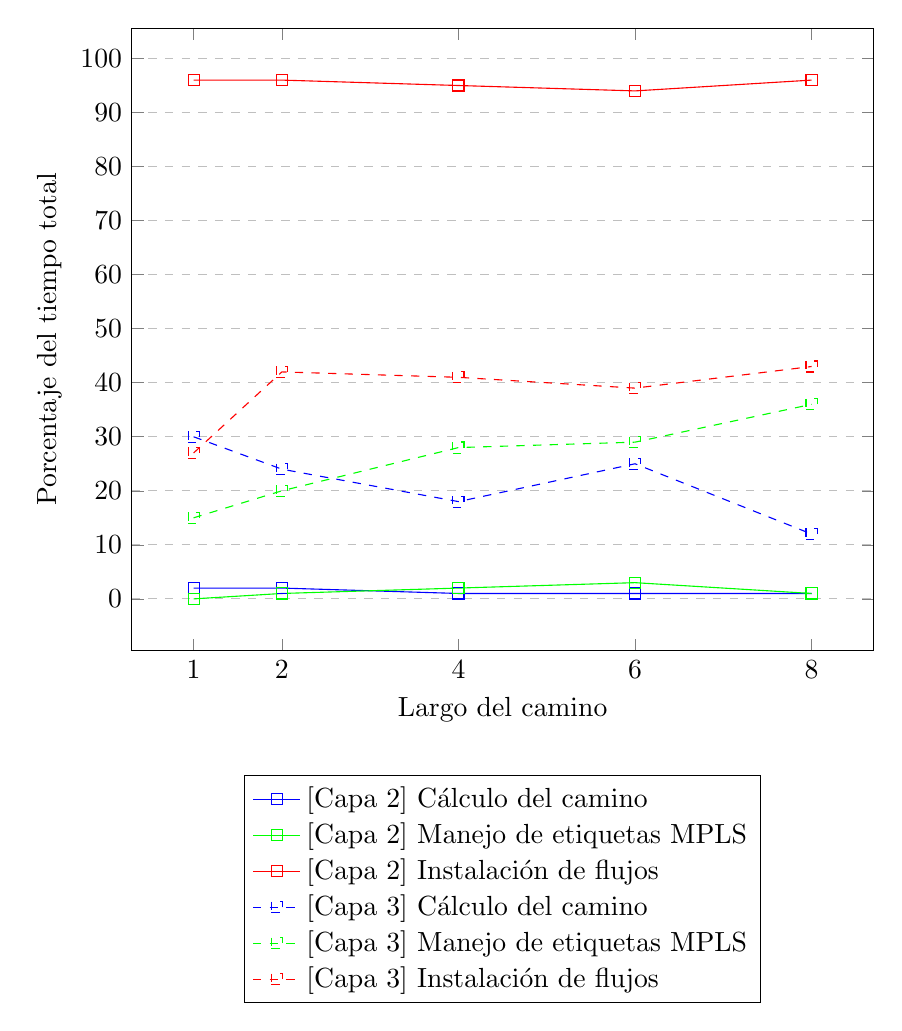
\begin{tikzpicture}
	\begin{axis}[
	xlabel={Largo del camino},
	ylabel={Porcentaje del tiempo total},
	xtick={0,1,2,4,6,8,10,12},
	ytick={0,10,20,30,40,50,60,70,80,90,100},
	scaled x ticks = false,
	x tick label style={/pgf/number format/fixed},
	legend style={at={(0.5,-0.2)},anchor=north},
	ymajorgrids=true,
	grid style=dashed,
	width=11cm,
	legend cell align=left,
	]
	\addplot[
	color=blue,
	mark=square,
	]
	coordinates {
		(1,2)(2,2)(4,1)(6,1)(8,1)
	};
	\addlegendentry{[Capa 2] Cálculo del camino}
	\addplot[
	color=green,
	mark=square,
	]
	coordinates {
		(1,0)(2,1)(4,2)(6,3)(8,1)
	};
	\addlegendentry{[Capa 2] Manejo de etiquetas MPLS}
	\addplot[
	color=red,
	mark=square,
	]
	coordinates {
		(1,96)(2,96)(4,95)(6,94)(8,96)
	};
	\addlegendentry{[Capa 2] Instalación de flujos}
	\addplot[
	color=blue,
	mark=square,
	dashed,
	]
	coordinates {
		(1,30)(2,24)(4,18)(6,25)(8,12)
	};
	\addlegendentry{[Capa 3] Cálculo del camino}
	\addplot[
	color=green,
	mark=square,
	dashed,
	]
	coordinates {
		(1,15)(2,20)(4,28)(6,29)(8,36)
	};
	\addlegendentry{[Capa 3] Manejo de etiquetas MPLS}
	\addplot[
	color=red,
	mark=square,
	dashed,
	]
	coordinates {
		(1,27)(2,42)(4,41)(6,39)(8,43)
	};
	\addlegendentry{[Capa 3] Instalación de flujos}
	\end{axis}
	\end{tikzpicture}
\end{figure}

Las gráficas en las figuras \ref{fig:gráfica_tiempo_chica}, \ref{fig:gráfica_tiempo_mediana} y \ref{fig:gráfica_tiempo_grande} muestran, para cada topología, cómo se descompone el tiempo de ejecución para cada largo de camino. Se omite la de la topología básica ya que sólo permite crear VPNs de largo 1. Cada punto en la gráfica indica el porcentaje del tiempo total que se necesitó para llevar a cabo una de las tres tareas ya mencionadas (cálculo del camino, manejo de etiquetas, instalación de flujos OpenFlow). Cada porcentaje se mide en base al promedio de 8 ejecuciones (descartando las ejecuciones que arrojan valores muy alejados del resto).

\begin{figure}[h]
	\caption{Distribución del tiempo de creación de VPNs en la topología mediana}
	\centering
	\label{fig:gráfica_tiempo_mediana}
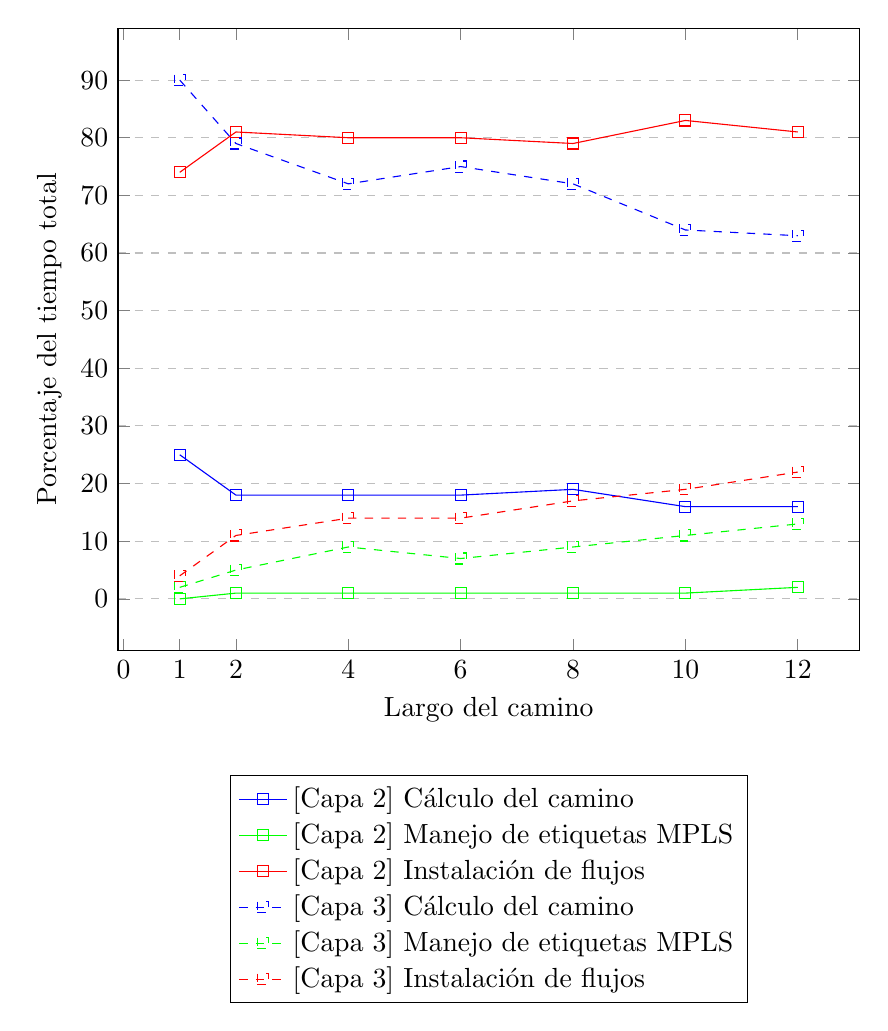
\begin{tikzpicture}
\begin{axis}[
xlabel={Largo del camino},
ylabel={Porcentaje del tiempo total},
xtick={0,1,2,4,6,8,10,12},
ytick={0,10,20,30,40,50,60,70,80,90,100},
scaled x ticks = false,
x tick label style={/pgf/number format/fixed},
legend style={at={(0.5,-0.2)},anchor=north},
ymajorgrids=true,
grid style=dashed,
width=11cm,
legend cell align=left,
]
\addplot[
color=blue,
mark=square,
]
coordinates {
	(1,25)(2,18)(4,18)(6,18)(8,19)(10,16)(12,16)
};
\addlegendentry{[Capa 2] Cálculo del camino}
\addplot[
color=green,
mark=square,
]
coordinates {
	(1,0)(2,1)(4,1)(6,1)(8,1)(10,1)(12,2)
};
\addlegendentry{[Capa 2] Manejo de etiquetas MPLS}
\addplot[
color=red,
mark=square,
]
coordinates {
	(1,74)(2,81)(4,80)(6,80)(8,79)(10,83)(12,81)
};
\addlegendentry{[Capa 2] Instalación de flujos}
\addplot[
color=blue,
mark=square,
dashed,
]
coordinates {
	(1,90)(2,79)(4,72)(6,75)(8,72)(10,64)(12,63)
};
\addlegendentry{[Capa 3] Cálculo del camino}
\addplot[
color=green,
mark=square,
dashed,
]
coordinates {
	(1,2)(2,5)(4,9)(6,7)(8,9)(10,11)(12,13)
};
\addlegendentry{[Capa 3] Manejo de etiquetas MPLS}
\addplot[
color=red,
mark=square,
dashed,
]
coordinates {
	(1,4)(2,11)(4,14)(6,14)(8,17)(10,19)(12,22)
};
\addlegendentry{[Capa 3] Instalación de flujos}
\end{axis}
\end{tikzpicture}
\end{figure}

\begin{figure}[h]
	\caption{Distribución del tiempo de creación de VPNs en la topología grande}
	\centering
	\label{fig:gráfica_tiempo_grande}
	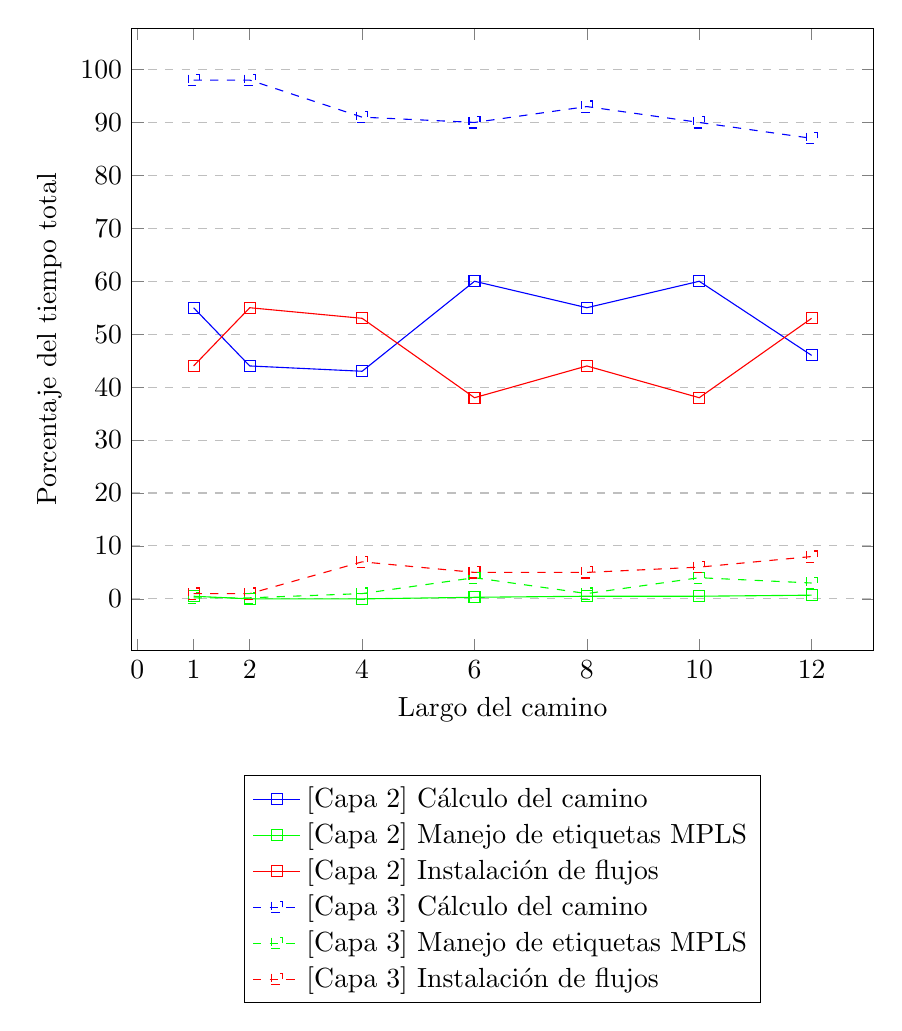
\begin{tikzpicture}
	\begin{axis}[
	xlabel={Largo del camino},
	ylabel={Porcentaje del tiempo total},
	xtick={0,1,2,4,6,8,10,12},
	ytick={0,10,20,30,40,50,60,70,80,90,100},
	scaled x ticks = false,
	x tick label style={/pgf/number format/fixed},
	legend style={at={(0.5,-0.2)},anchor=north},
	ymajorgrids=true,
	grid style=dashed,
	width=11cm,
	legend cell align=left,
	]
	\addplot[
	color=blue,
	mark=square,
	]
	coordinates {
		(1,55)(2,44)(4,43)(6,60)(8,55)(10,60)(12,46)
	};
	\addlegendentry{[Capa 2] Cálculo del camino}
	\addplot[
	color=green,
	mark=square,
	]
	coordinates {
		(1,0.5)(2,0)(4,0)(6,0.3)(8,0.5)(10,0.5)(12,0.7)
	};
	\addlegendentry{[Capa 2] Manejo de etiquetas MPLS}
	\addplot[
	color=red,
	mark=square,
	]
	coordinates {
		(1,44)(2,55)(4,53)(6,38)(8,44)(10,38)(12,53)
	};
	\addlegendentry{[Capa 2] Instalación de flujos}
	\addplot[
	color=blue,
	mark=square,
	dashed,
	]
	coordinates {
		(1,98)(2,98)(4,91)(6,90)(8,93)(10,90)(12,87)
	};
	\addlegendentry{[Capa 3] Cálculo del camino}
	\addplot[
	color=green,
	mark=square,
	dashed,
	]
	coordinates {
		(1,0.2)(2,0.2)(4,1)(6,4)(8,1)(10,4)(12,3)
	};
	\addlegendentry{[Capa 3] Manejo de etiquetas MPLS}
	\addplot[
	color=red,
	mark=square,
	dashed,
	]
	coordinates {
		(1,1)(2,1)(4,7)(6,5)(8,5)(10,6)(12,8)
	};
	\addlegendentry{[Capa 3] Instalación de flujos}
	\end{axis}
	\end{tikzpicture}
\end{figure}

Las líneas rojas muestran como evoluciona el porcentaje del tiempo que abarca la instalación de flujos. Se observa que la porción de tiempo requerida para la instalación de los flujos de una VPN de capa 2 (denotada por las líneas rojas continuas) queda siempre por encima de la requerida para instalar flujos de una VPN de capa 3 (líneas rojas punteadas). Esto se debe a que, como ya fue explicado anteriormente, una VPN de capa 2 debe instalar más flujos en los nodos, lo cual implica que se debe dedicar más tiempo a la etapa de instalación de flujos. Para ambos tipos de VPN se observa que la instalación de flujos abarca más tiempo de ejecución (las líneas suben) a medida que el camino es más largo. Esto es esperable ya que más nodos implican más flujos. Curiosamente, esta suba parece ser más pronunciada para la VPN de capa 3.

Las líneas verdes muestran qué porcentaje del tiempo total se dedica al cálculo y manejo de etiquetas MPLS. Igual que la instalación de flujos, esta etapa requiere más tiempo a medida que hay más nodos en el camino, ya que se aumenta la cantidad de etiquetas MPLS. También se observa que la VPN de capa 3 requiere un mayor porcentaje del tiempo que la de capa 2 para esta tarea. Esto puede resultar extraño, ya que la de capa 2 debe manejar más etiquetas. Lo que ocurre es que la de capa 2 requiere más tiempo absoluto, pero el tiempo total de creación de la VPN también es mayor, por lo tanto el porcentaje del tiempo que se dedica a la tarea resulta mayor para la VPN de capa 3. Otra observación es que esta tarea es la que menos tiempo requiere de las tres.

Por último, el cálculo del camino óptimo. Lo primero a tener en cuenta es que esta etapa no es afectada por el tipo de VPN que se está creando, ya que lo único que debe hacer es determinar el camino óptimo entre dos nodos de un grafo. Tampoco es afectada por el largo del camino que está calculando. Lo único que la afecta es el tamaño de la topología.
Las líneas azules denotan la participación del cálculo del camino óptimo en la distribución del tiempo. Lo primero que se observa es que el porcentaje de tiempo dedicado a esta tarea decrece a medida que se aumenta el largo del camino. Esto es esperable, ya que el tiempo requerido tiende a ser constante, mientras que las otras tareas requieren más tiempo, por lo tanto su porción del tiempo disminuye. Otra observación interesante es que a medida que se aumenta el tamaño de la topología, esta etapa ocupa una mayor parte del tiempo de ejecución. En la topología chica la etapa de instalación de flujos se lleva la mayor parte del tiempo de ejecución tanto para la VPN de capa 2 como la de capa 3. Sin embargo, en la topología mediana eso cambia, y se cumple sólo para la VPN de capa 2. Por último, en la topología grande, ya no se observa eso para ninguno de los dos tipos, y la VPN de capa 2 reparte de forma bastante equitativa el tiempo de ejecución entre el cálculo del camino y la instalación de flujos.

Desde el punto de vista técnico esto también es esperable, ya que el algoritmo que calcula el camino es de orden cuadrático en la cantidad de nodos, mientras que las otras etapas (manejo de etiquetas e instalación de flujos OpenFlow) aumentan linealmente con la cantidad de nodos en el camino. Esto lleva a creer que si se siguiera experimentando con topologias aún más grandes, el cálculo del camino óptimo eventualmente abarcaría la mayoría del tiempo de creación de las VPNs, tanto de capa 2 como de capa 3.


\section{Escala de servicios y flujos}
Entre los requerimientos de la RAU2 se encuentra el de la escalabilidad de usuarios. Específicamente, se espera alcanzar en un mediano plazo un total de 11.000 docentes, 7.000 funcionarios y 140.000 estudiantes (de acuerdo a los requerimientos relevados por el proyecto RRAP). Esto implica que la red será sujeta a importantes cantidades de servicios y flujos distintos. Para poder asegurar que la arquitectura escala sin problemas, se la debería someter a experimentos que reflejen los niveles de actividad y tráfico que son esperados en un futuro. Sin embargo, dichos experimentos no son llevados a cabo por este trabajo por dos razones. En primer lugar, se considera que es una tarea que lleva demasiado tiempo como para ser incluida dentro del alcance de este trabajo. En segundo lugar, no están disponibles los modelos y patrones de tráfico que serían necesarios para esas pruebas.

También es importante recordar que el entorno virtual no generará resultados relevantes en lo que refiere al nivel real de rendimiento de la arquitectura. Utilizar un emulador significa que los recursos de la computadora se repartirán entre todos los nodos virtuales, por lo tanto el rendimiento que se observe en la red emulada será inferior al observado en una red física.

Se puede concluir entonces que las pruebas detalladas a continuación no aseguran la escalabilidad de RAUFlow, pero sí ayudan a investigar el comportamiento de la red y los dispositivos cuando se los somete a muchos servicios.

\subsection{Descripción del escenario}
El escenario de prueba consiste en crear una cantidad relativamente grande de VPNs en la topología básica, y analizar si esto degrada el rendimiento de la red de alguna forma. Se utiliza una VPN punto a punto de capa 3 para conectar dos subredes cliente, y se utiliza \textit{iperf} para generar tráfico TCP y medir el ancho de banda entre los dos hosts. Para cargar al controlador con servicios, se crean múltiples VPN de capa 2 entre las subredes, variando los valores de los cabezales VLAN\_ID y VLAN\_PCP (pudiendo crear un total de 32.768 combinaciones distintas) para que toda VPN sea distinta de las demás. De esta forma, existirán múltiples VPN pero solo una (la de capa 3) será utilizada con tráfico. \\
Dado que cargar todas las VPN a mano en la interfaz web llevaría demasiado tiempo, se creó un servicio web que recibe como parámetro la cantidad de VPN que se desean. Cuando se hace un pedido GET a ese servicio web, se inicia el proceso de creación de las mismas. Este proceso puede tomar entre algunos minutos y varias horas, dependiendo de la cantidad. \\ \\
Con este escenario de prueba se busca verificar los dos siguientes aspectos claves: \\ \\
\textbf{Escalabilidad interna del RAUSwitch} \\
Se estudian posibles limitaciones internas que puedan tener los dispositivos cuando deben manejar grandes cantidades de flujos. Es posible que a medida que crecen sus tablas de flujos, demoren más en encontrar el flujo que se corresponde con cada paquete que reciben. Si pasa esto, el throughput debería ser afectado negativamente por la cantidad de flujos en sus tablas.
\textbf{Escalabilidad en servicios} \\
Se estudian posibles problemas que puedan tener la arquitectura de la red o, en particular, la aplicación RAUFlow para manejar grandes cantidades de servicios o información. Es de particular interés medir la memoria que requiere el controlador para mantener los servicios. \\ \\

\subsection{Resultados y observaciones}

\begin{table}[ht]
	\caption{Throughput en Kbits/s medidos para distintas cantidades de VPNs.}
	\centering 
	\begin{tabular}{c c}
		\hline\hline
		\# de VPNs & Throughput (Kbits/s) \\ [0.5ex]
		\hline
		1 & 1287 \\
		3000 & 1286 \\
		6000 & 1265 \\
		9000 & 1270 \\
		12000 & 1290 \\
		15000 & 1280 \\ [1ex]
		\hline
	\end{tabular}
	\label{table:escala_de_servicios}
\end{table}

Como se explica en la descripción del escenario, se busca determinar si la existencia de muchos flujos en la tabla implica que un RAUSwitch demora más tiempo en encontrar el flujo OpenFlow que corresponde para un paquete entrante, y por lo tanto demora más en determinar la acción a tomar para ese paquete. Si esto fuera así, debería existir una relación inversamente proporcional entre la cantidad de flujos en la tabla de un nodo y su velocidad para procesar paquetes. En la tabla \ref{table:escala_de_servicios} se pueden observar los throughput promedio medidos para un flujo de datos sobre la topología básica, con distintas cantidades de VPN existiendo en la red. La principal conclusión que se puede sacar de la tabla es que el throughput no es afectado por la cantidad de VPNs existentes en el momento (se asume que las pequeñas diferencias numéricas entran en el margen de error).

Se puede ver que la máxima cantidad de VPNs con la que se probó fue de 15.000. Cada VPN de capa 2 está compuesta por dos servicios de capa 2, y cada uno de esos servicios introduce 42 flujos en cada nodo del camino. Esto quiere decir que cada uno contiene alrededor de 1.260.000 (15.000 * 2 * 42) flujos en su tabla. Se podría argumentar que hacen falta más flujos para impactar el throughput, pero en realidad la explicación se encuentra en la especificación de Open vSwitch, y ya fue mencionada en el capítulo 2. Open vSwitch realiza cacheo de flujos. Eso quiere decir que cuando un paquete de datos de un determinado flujo llega por primera vez a un nodo, este paquete es enviado al pipeline de OpenFlow para determinar qué acción se debe tomar. Luego de realizada, esta acción es escrita en la caché, y tiene un tiempo de vida de entre 5 y 10 segundos. Si en ese período de tiempo llega otro paquete del mismo flujo, no hay necesidad de enviar el paquete al pipeline, porque ya se sabe cuales son las acciones a tomar para el mismo. Por lo tanto, si un flujo de datos es constante y rápido, el tamaño de la tabla de OpenFlow no afectará el tiempo de decisión, ya que sólo el primer paquete de ese flujo deberá ser comparado con dicha tabla. La figura \ref{fig:ovs_dataplane} ilustra este comportamiento.

\begin{figure}[t]
	\caption{Arquitectura simplificada de Open vSwitch.}
	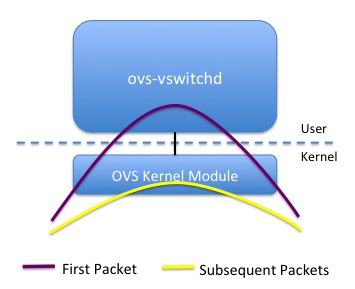
\includegraphics[scale=0.65]{ovs_dataplane}
	\centering
	\label{fig:ovs_dataplane}
\end{figure}

Mediante el comando "ovs-dpctl show" de Open vSwitch, se puede examinar las estadísticas de la cache de cada nodo. A modo de ejemplo, en la figura \ref{fig:cache_sample} se observan las estadísticas de un nodo llamado "alice". En la sección "lookups" se detallan cuantos "hits" y "miss" de caché han ocurrido hasta el momento, y "flows" indica cuantos flujos activos hay en el momento en la caché.

\begin{figure}[H]
	\caption{Estadísticas de cache de flujos del nodo "alice".}
	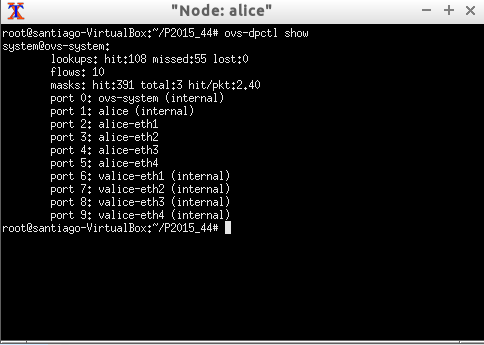
\includegraphics[scale=1]{cache_sample}
	\centering
	\label{fig:cache_sample}
\end{figure}

Otro objetivo de la prueba es determinar si la arquitectura, y en particular el controlador, tienen algún problema para manejar muchos servicios. No se ha detectado ningún problema de esa índole. Sin embargo, es importante recordar que el controlador mantiene toda su información en memoria, por lo tanto es de interés realizar un estudio del consumo de memoria del mismo a medida que crece la cantidad de servicios. El comando de Linux llamado \textit{pmap} permite estudiar el consumo de memoria del proceso que se le indique, y con el mismo se puede analizar la evolución del consumo de memoria del controlador a medida que se le agregan servicios. En la tabla \ref{table:consumo_de_memoria} y la figura \ref{fig:consumo_de_memoria} se puede observar el resultado de estas mediciones. \\

\begin{table}[ht]
	\caption{Evolución del consumo de memoria del controlador.}
	\centering 
	\begin{tabular}{c c}
		\hline\hline
		\# de VPNs & Memoria (KB) \\ [0.5ex]
		\hline
		0 & 33280 \\
		3000 & 108196 \\
		6000 & 182460 \\
		9000 & 256528 \\
		12000 & 333244 \\
		15000 & 407696 \\ [1ex]
		\hline
	\end{tabular}
	\label{table:consumo_de_memoria}
\end{table}

\begin{figure}
\caption{Efecto de la cantidad de VPN sobre la memoria consumida}
\centering
\label{fig:consumo_de_memoria}
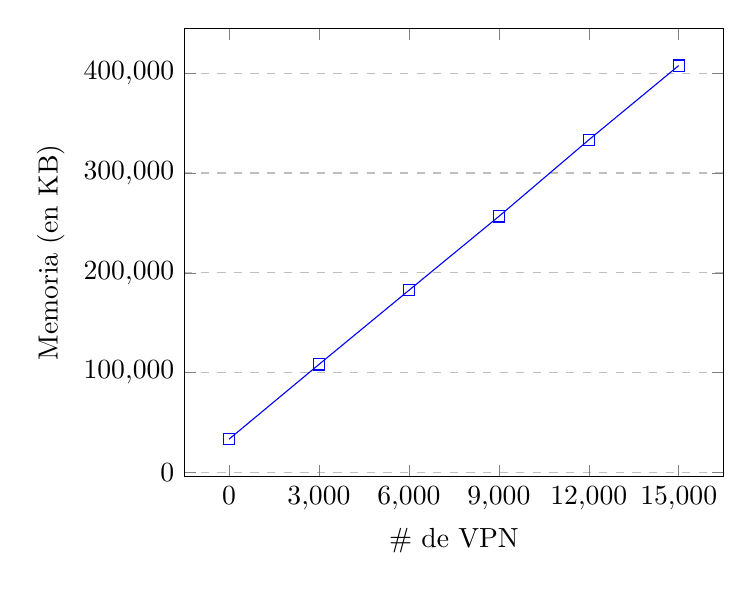
\begin{tikzpicture}
\begin{axis}[
xlabel={\# de VPN},
ylabel={Memoria (en KB)},
xtick={0,3000,6000,9000,12000,15000},
ytick={0,100000,200000,300000,400000,500000},
scaled x ticks = false,
scaled y ticks = false,
x tick label style={/pgf/number format/fixed},
y tick label style={/pgf/number format/fixed},
legend pos=north west,
ymajorgrids=true,
grid style=dashed,
]
\addplot[
color=blue,
mark=square,
]
coordinates {
	(0,33280)(3000,108196)(6000,182460)(9000,256528)(12000,333244)(15000,407696)
};
\end{axis}
\end{tikzpicture}
\end{figure}

La principal observación que se puede hacer es que el consumo de memoria del controlador aumenta de forma lineal con la cantidad de servicios. El mismo se incrementa en 74916 KB cada 3000 servicios, por lo tanto se puede calcular que cada servicio ocupa alrededor de 25 KB (74916/3000). A modo de ejemplo, si extrapolamos ese número a una computadora que puede dedicar 4 Gb de RAM para mantener los servicios, llegamos a que el controlador podrá mantener alrededor de 167.772 servicios. A pesar de que no es ideal mantener tantos datos en memoria, se puede concluir que es un consumo aceptable. \\

En el proceso de realizar las pruebas ya mencionadas también se observó un comportamiento que no se esperaba. Se detectó que a medida que hay más VPNs creadas, la red demora más tiempo en crear una nueva VPN. Con el propósito de entender más ese comportamiento, se hizo un experimento cuyos resultados se observan en la figura \ref{fig:tiempo_vpns_acumuladas}.

\begin{figure}
\caption{Efecto de la cantidad de VPNs sobre el tiempo de carga de una VPN nueva}
\centering
\label{fig:tiempo_vpns_acumuladas}
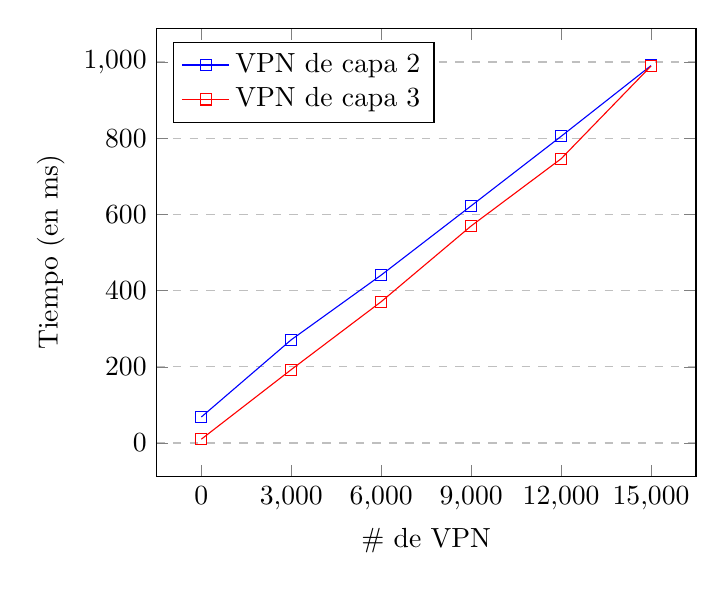
\begin{tikzpicture}
\begin{axis}[
xlabel={\# de VPN},
ylabel={Tiempo (en ms)},
xtick={0,3000,6000,9000,12000,15000},
ytick={0,200,400,600,800,1000,1200},
scaled x ticks = false,
x tick label style={/pgf/number format/fixed},
legend pos=north west,
ymajorgrids=true,
grid style=dashed,
]
\addplot[
color=blue,
mark=square,
]
coordinates {
	(1,68.2)(3000,270.9)(6000,440.7)(9000,622.4)(12000,804.8)(15000,990.5)
};
\addlegendentry{VPN de capa 2}
\addplot[
color=red,
mark=square,
]
coordinates {
	(1,10.0)(3000,192.6)(6000,370.9)(9000,569.6)(12000,746.0)(15000,989.3)
};
\addlegendentry{VPN de capa 3}
\end{axis}
\end{tikzpicture}
\end{figure}

Cada punto indica el tiempo que demora la red en dar de alta una nueva VPN con una determinada cantidad de VPN ya existentes. Estos tiempos se miden de la misma forma que los obtenidos en la sección de pruebas anterior: se toma el tiempo que demora la aplicación en devolver la respuesta HTTP indicando que el servicio se creó con éxito (disponible en los logs). En la gráfica se puede ver que el tiempo de carga aumenta de forma lineal a medida que hay más VPN en la red, y esto se cumple para la de capa 2 como la de capa 3. Una posible explicación inicial para esto puede ser que al tener más flujos, cada nodo demora más en insertar nuevos flujos en su tabla. Esa teoría se descarta con el siguiente razonamiento. En la gráfica se observa que toma más tiempo crear una VPN de capa 2 que una de capa 3. Esto en gran medida se explica porque un servicio de capa 2 debe insertar 42 flujos en los nodos del camino, mientras que uno de capa 3 solo inserta 1. Pero también se observa que las lineas son virtualmente paralelas, es decir, esa diferencia de tiempo se mantiene constante a pesar de las VPNs que existan. Si insertar un flujo nuevo cada vez tomara más tiempo, ese incremento se debería multiplicar por 42 para la VPN de capa 2, y la linea correspondiente a la VPN de capa 2 debería tener una pendiente más inclinada que la de capa 3.

Otra posible explicación para este comportamiento, y quizás la más probable, es que la aplicación RAUFlow se vuelve más lenta a medida que sus estructuras de datos crecen. Sin embargo, no se observa ninguna característica en el código que indique esto.
